% Preamble
% ---
\documentclass[a4paper,13pt]{article}
\usepackage[utf8]{inputenc}
\usepackage{amsmath}
\usepackage{graphicx}
\usepackage{lipsum}
\usepackage{fancyhdr}
\usepackage{lastpage}
\usepackage[margin=0.8in]{geometry}
\numberwithin{equation}{section}
\pagestyle{fancy}
\fancyhf{}
\rhead{AnkushB}
\lhead{LaTeX - Test1}
\cfoot{\thepage-\pageref{LastPage}}
\newcommand\eqline[1]{\begin{equation} #1 \end{equation}}
\newcommand\hfrac{\frac{\hbar^2}{2m}}
\newcommand\dif[2]{\frac{d #1}{d #2}}
\newcommand\diff[2]{\frac{d^2 #1}{d #2^2}}
\newcommand\oneby[1]{\frac{1}{#1}}
\newcommand\pdif[2]{ \frac{\partial #1}{\partial #2}}
\newcommand\sun{\cdot}
\title{Test Document one}
\author{AnkushB}
\begin{document}
\maketitle
\begin{abstract}
This is the abstract of the document, everything important goes here.
\end{abstract}
\tableofcontents{}
\paragraph{Introduction}
This is a test document saofnacd ecw, This doesn't seem to have spell check. 
Next line with enter. Enter doesnt change the line, nor does it alter the formatting in any way.
This paragraph is full of bullshit text to check whether this changes to new line automatically after the line exceeds the margins. This should do the trick... Apparently it does, but now the margins are shit wide.
\paragraph{Para2}
This is the second paragraph, test 2 para 2 with a 
\paragraph {}
New Paragraph which has different things such as new stuff that goes into the next paragraph, also the formatting that is the same as the previous paragraph. I love typing hence I'm typing gibberish just for test. Now these are my first equations:
\begin{align}
f(x) &= x^2\\
f'(x) &= 2x\\
F(x) &= \int f(x)dx\\
F(x) &= \frac{1}{3}x^3  %no spaces remember
\end{align}
This is the paragraph after the equations. 
\section{This is section one}
This is the words of section one. I am trying to learn Latex as fast as possible so that I can start writing my own paper. I would put random stuff about my own things in here.
\begin{align}
f(x) &= ax^2+bx+c\\
\int f(x,y)dxdy\ &= \int^{a}_{b} \frac{f(y)}{n+1}x^{n+1} dy\\
\end{align}
\subsection{This is sub section number one}
This is my first subsection, I will put random things here as well. This is just to fill in this section with some paragraphs/words.
\subsection{This is the second sub section}
Fliier text made up of random words that help me type without looking at the keyboard.
\subsubsection{This is sub sub section}
This is just filler text for the sub sub section. This doesn't mean shit, Just there to fill up some space for the text.
\paragraph{This is para two}
This is just some filler text for some tex stuff. I dont mean shit with this thing, Just filling up and trying to learn how it looks at the output.
\subparagraph{This is the subpara}
Hello from the other side......\\
This is the linebreak thingie, I can Line brake with two slashes \\ like that
\section{Section of the pictures :D}
This is the section after the figure. Please see to it that it prints after the figure
\begin{figure}
  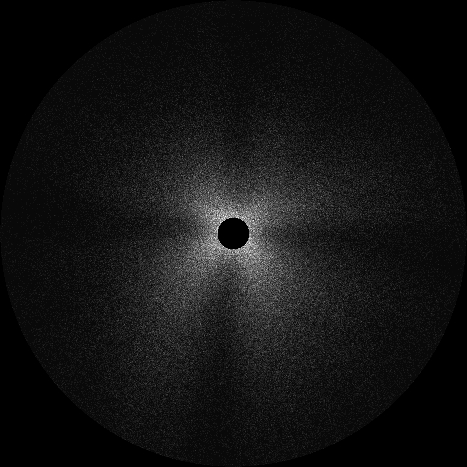
\includegraphics[width=400]{PCP4_1am.jpg}
  \caption{This is the PC mode 1am Exclusion data}
  \label{fig:PC_1am}
\end{figure}
\end{document}